\documentclass{article}
\usepackage[utf8]{inputenc}
\usepackage{bbm} 
\usepackage{tabularx}
\usepackage{amsopn}
\usepackage{amsmath}
\usepackage{amsfonts}
\usepackage{hyperref}
\usepackage{tikz}
\usepackage{pgfplots}

\usepackage{bm}
\title{%
   Homework 2 \\
  \large Fondations of Machine Learning \\}
\author{Xiang Pan (xp2030)}

\begin{document}


\maketitle
\section*{VC Dimension}
\section{}
\subsection*{(a)}
Show that there exists a set of $n+1$ points in $\mathbb{R}^{n}$ that can be shattered by $\mathcal{B}_{n}$. Conclude that VCdim $\left(\mathcal{B}_{n}\right) \geq n+1$


We have n+1 points can determine a unique ball in $\mathbb{R}^{n}$, and we have the ball center c, radius r. 

For those negative points $p_n \in P_{N}$, we have the radius from $p_n$ to c, thus we can constuct the new $p_n' = p_n + \delta(c-p_n)$.
$\delta>0$. Thus we can constuct a new ball with new n+1 points set ${P_N'} \bigcup {P_P}$. For the new ball B(c', r'), the negative points distance $r>r'$, the positive points $r'\leq r'$. Thus B(c', r') can shatter n+1 points in $\mathbb{R}^{n}$.

For $r > r'$, the B(c,r) and B(c',r') are joint, since $P_P$ are in the B(c,r) and B(c',r'). Note that, $P_N'$ are strictly inside B(c,r), it is easy to check that $P_N$ are strictly outside B(c',r'). 

\subsection*{(b)}

Let $B(c, r)$ be the ball of radius $r$ centered at $c \in \mathbb{R}^{n}$. Then $x \in B(c, r)$ 

\begin{equation}
\left\| x - c \right\|^2 \leq r
\end{equation}


\begin{equation}
\sum_{i=1}^{n}\left\|x_{i}\right\|^{2}-2 \sum_{i=1}^{n} c_{i} x_{i}+\sum_{i=1}^{n} c_{i}^{2}-r \leq 0
\end{equation}

We can find a hyperplane $h$ that is orthogonal to $B(c, r)$ and $x$ is in $B(c, r)$ if $h \cdot x' + b \leq 0$.

\begin{align}
    h = 
    \begin{bmatrix}
        1,      \\
        -2c_{1},\\
        -2c_{2},\\
        \cdot   \\
        -2c_{n} \\
    \end{bmatrix}
\end{align}


\begin{align}
    x' =
    \begin{bmatrix}
        \sum_{i=1}^{n} {\|x_{i}\|}^2 \\
        x_{1} \\
        x_{2} \\
        \cdot \\
        x_{n} \\
    \end{bmatrix}
\end{align}


\begin{align}
    b = \sum c_{i}^{2} - r
\end{align}

The VC dimension of $B(c, r)$ is at most as the same as the VC dimension of hyperplane $R^{n+1}$, which is n+2.


\subsection*{(c)}
Show that VCdim 
\begin{equation}
    \left(\mathcal{B}_{2}\right)=3 \text {. }
\end{equation}

We have already know that 

\begin{align}
    3 \leq \left(\mathcal{B}_{2}\right) \leq 4
\end{align}

But for four points, 

\begin{center}
    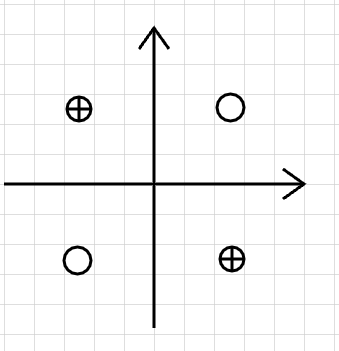
\includegraphics[width=100px]{./images/1_1.png}
\end{center}


This case can not find a ball to shatter it.

Thus we have VCdim $\left(\mathcal{B}_{2}\right) = 3$

\section*{Maximum Margin Multiple Kernel}
\section*{1}
\subsection*{(a)}

\begin{equation}
    \widehat{\mathcal{M}}_{q}=\left\{\boldsymbol{\mu}: \boldsymbol{\mu} \in \Delta_{q}, \widehat{\gamma}_{K_{\mu}} \geq \gamma_{0}\right\}
\end{equation}

$\Delta_q$ is the set of $\mu$,

\begin{equation}
    \Delta_{q}=\left\{\boldsymbol{\mu}: \boldsymbol{\mu} \geq 0,\|\boldsymbol{\mu}\|_{q}=1\right\} \text { with } q \geq 1
\end{equation}

K is the combined kernel function, $\mu$ is the weight for each kernel component,

\begin{equation}
    K = \sum_{k=1}^{p} \mu_{k} K_{k}
\end{equation}

To explain $\gamma$, we need to show where the $\gamma_0$ from.

From the paper,
\begin{equation}
    \max _{\boldsymbol{\mu} \in \Delta_{q}} \sum_{i=1}^{m} \min _{y \neq y_{i}} \boldsymbol{\mu} \cdot \boldsymbol{\eta}\left(x_{i}, y_{i}, y\right)
\end{equation}

which equals to 

\begin{equation}
    \max _{\boldsymbol{\mu} \in \Delta_{q}} \frac{1}{m} \sum_{i=1}^{m} \min _{y \neq y_{i}} \boldsymbol{\mu} \cdot \boldsymbol{\eta}\left(x_{i}, y_{i}, y\right)
 \end{equation}.

Converting the optimization to convex optimization, we have

 \begin{equation}
    \max _{\substack{\mu \in \Delta_{q} \\ \gamma}} \sum_{i=1}^{m} \gamma_{i} \text { s.t. } \forall i \in[1, m], \forall y \neq y_{i}, \boldsymbol{\mu} \cdot \boldsymbol{\eta}\left(x_{i}, y_{i}, y\right) \geq \gamma_{i}
\label{eq:max_margin_convex}
\end{equation}


We can directly solve the optimization problem, however we can convert it to a minimization problem with constraint $\widehat{\gamma}_{K_{\boldsymbol{\mu}}} \geq \gamma_{0}$.

\begin{equation}
    \widehat{\gamma}_{K_{\mu}}=\frac{1}{m} \sum_{i=1}^{m} \min _{y \neq y_{i}} \boldsymbol{\mu} \cdot \boldsymbol{\eta}\left(x_{i}, y_{i}, y\right)
\end{equation}

For $\gamma_0$, setting it equal to the maximum feasible value will guarantee that the selected $\bm{\mu}$ is also give us the solution as \eqref{eq:max_margin_convex}.

\subsection*{(b)}

\begin{equation}
    \begin{aligned}
        \min _{\boldsymbol{\mu} \in \widehat{\mathcal{M}}_{q}} \min _{\mathbf{w}, \boldsymbol{\xi}} &\frac{1}{2} \sum_{y=1}^{c} \sum_{k=1}^{p} \frac{\left\|\mathbf{w}_{y, k}\right\|^{2}}{\mu_{k}}+C \sum_{i=1}^{m} \xi_{i}, \\
        \text{subject to: } &\forall i \in[1, m], \xi_{i} \geq 0, \forall y \neq y_{i} \\
        &\xi_{i} \geq 1-\left(\mathbf{w}_{y_{i}} \cdot \Phi\left(x_{i}\right)-\mathbf{w}_{y} \cdot \Phi\left(x_{i}\right)\right)
    \end{aligned}
\end{equation}




We can derive the Lagrangian Function as
\begin{align}
    \begin{aligned}
        \mathcal{L}(\mathbf{w}, \boldsymbol{\xi}, \bm{\alpha}, \bm{\beta}) 
        &= \frac{1}{2} \sum_{y=1}^{c} \sum_{k=1}^{p} \frac{\left\|\bm{w}_{y, k}\right\|^{2}}{\mu_{k}}
        + C \sum_{i=1}^{m} \xi_{i} \\
        &- \sum_{i=1}^{m} 
           \sum_{y \neq y_i}
            \alpha_{i, y}
            \left(
                \bm{w}_{y_{i}} \cdot \Phi\left(x_{i}\right)
                - \bm{w}_{y} \cdot \Phi\left(x_{i}\right) 
                + \xi_{i}
                - 1
            \right)
        - \sum_{i=1}^{m} \beta_{i} \xi_{i} 
    \end{aligned}
\end{align}

\begin{align}
    \begin{aligned}
        \mathcal{L}(\mathbf{w}, \boldsymbol{\xi}, \bm{\alpha}, \bm{\beta}) 
        &= \frac{1}{2} \sum_{y=1}^{c} \sum_{k=1}^{p} \frac{\left\|\bm{w}_{y, k}\right\|^{2}}{\mu_{k}}
        + C \sum_{i=1}^{m} \xi_{i} \\
        &- \sum_{i=1}^{m} 
            \sum_{y \neq y_i}
            \alpha_{i, y}
            \left(
                \bm{w}_{y_{i}} \cdot \Phi\left(x_{i}\right)
                + \xi_{i} - 1
            \right)\\
        &+ \sum_{i=1}^{m} 
        \sum_{y \neq y_i}
        \alpha_{i, y} \bm{w}_{y} \cdot \Phi\left(x_{i}\right) \\
        &- \sum_{i=1}^{m} \beta_{i} \xi_{i}
    \end{aligned}
\end{align}

% We define,
% \begin{equation}
%     W' = 
% \end{equation}



m is the dataset size, c is the number of classes, p is the number of kernel components.

Using KKT,
\begin{align}
    \begin{aligned}
        \nabla_{\bm{w}_{y, k}} \mathcal{L} = 
        \frac{\bm{w}_{y, k}}{\mu_k} - 
         \sum_{i: y_i = y} \sum_{y' \neq y} \alpha_{i, y'} \Phi_k(x_i)
        +\sum_{i: y_i \neq y}   \alpha_{i, y} \Phi_k(x_i) = 0
    \end{aligned} \\
    \quad \Longrightarrow \quad
    w_{y, k} = 
    \mu_k
    \left(
        \sum_{i: y_i = y} \sum_{y' \neq y} \alpha_{i, y'} \Phi_k(x_i) -\sum_{i: y_i \neq y}  \alpha_{i, y} \Phi_k(x_i)
    \right) \\
    \mu_k
    \left(
        \sum_{i: y_i = y} \Phi_k(x_i) 
        \sum_{y' \neq y} \alpha_{i, y'}  -\sum_{i: y_i \neq y}  \alpha_{i, y} \Phi_k(x_i) 
    \right) \\
    \mu_k
    \left(
        \sum_{i: y_i = y} \Phi_k(x_i) 
        ((\sum_{y''} \alpha_{i, y''}) - \alpha_{i, y})) 
        -\sum_{i: y_i \neq y}  \alpha_{i, y} \Phi_k(x_i) 
    \right) \\
    \mu_k
    \left(
        \sum_{i: y_i = y} \Phi_k(x_i) 
        \sum_{y''} \alpha_{i, y''}
        -\sum_{i: y_i = y}   \alpha_{i, y} \Phi_k(x_i)
        -\sum_{i: y_i \neq y}  \alpha_{i, y} \Phi_k(x_i) 
    \right) \\
    \mu_k
    \left(
        \sum_{i: y_i = y} \Phi_k(x_i) 
        \sum_{y''} \alpha_{i, y''}
        -\sum_{i=1}^{m}   \alpha_{i, y} \Phi_k(x_i)
    \right) 
\end{align}


\begin{equation}
    \nabla_{\xi_{i}} \mathcal{L}=C- \sum_{y \neq y_i} \alpha_{i,y}- \beta_{i}=0 
    \quad \Longrightarrow \quad 
    \sum_{y \neq y_i}\alpha_{i, y}+\beta_{i}=C
\end{equation}

\begin{equation}
    \begin{aligned}
        \forall {i} \wedge \{y \neq y_i\},
        \alpha_{i, y}
        \left(
            \bm{w}_{y_{i}} \cdot \Phi\left(x_{i}\right)
            - \bm{w}_{y} \cdot \Phi\left(x_{i}\right) 
            + \xi_{i}
            - 1
        \right) = 0 \\
        \quad \Longrightarrow \quad 
        \alpha_{i, y} = 0 \vee
        \left[
            \left(
                \bm{w}_{y_{i}} \cdot \Phi\left(x_{i}\right)
                - \bm{w}_{y} \cdot \Phi\left(x_{i}\right)
            \right)
            = 1 - \xi_{i}
        \right]
    \end{aligned}
\end{equation}

\begin{equation}
    \forall i, \beta_{i} \xi_{i}=0 \quad \Longrightarrow \quad \beta_{i}=0 \vee \xi_{i}=0
\end{equation}



Using the KKT condition,
\begin{align}
    \begin{aligned}
        \mathcal{L}(\mathbf{w}, \boldsymbol{\xi}, \bm{\alpha}, \bm{\beta}) 
        &= \frac{1}{2} \sum_{y=1}^{c} \sum_{k=1}^{p} \frac{\left\|\bm{w}_{y, k}\right\|^{2}}{\mu_{k}}
        + C \sum_{i=1}^{m} \xi_{i} \\
        &- \sum_{i=1}^{m} 
           \sum_{y \neq y_i}
            \alpha_{i, y}
            \left(
                \bm{w}_{y_{i}} \cdot \Phi\left(x_{i}\right)
                - \bm{w}_{y} \cdot \Phi\left(x_{i}\right) 
                + \xi_{i}
                - 1
            \right)
        - \sum_{i=1}^{m} \beta_{i} \xi_{i} 
    \end{aligned}
\end{align}


\begin{equation}
    \frac{1}{2} \sum_{y=1}^{c} \sum_{k=1}^{p} \frac{\left\|\mathbf{w}_{y, k}\right\|^{2}}{\mu_{k}}+C \sum_{i=1}^{m} \xi_{i} - \sum_{i=1}^{m} 
    \sum_{y \neq y_i}
     \alpha_{i, y}
     \left(
         \bm{w}_{y_{i}} \cdot \Phi\left(x_{i}\right)
         - \bm{w}_{y} \cdot \Phi\left(x_{i}\right) 
         + \xi_{i}
         - 1
     \right)
 - \sum_{i=1}^{m} \beta_{i} \xi_{i} 
\end{equation}

\begin{equation}
    \frac{1}{2} \sum_{y=1}^{c} \sum_{k=1}^{p} \frac{\left\|\mathbf{w}_{y, k}\right\|^{2}}{\mu_{k}}+C \sum_{i=1}^{m} \xi_{i} - 
    \sum_{i=1}^{m} 
    \sum_{y \neq y_i}
     \alpha_{i, y}
    \sum_{k=1}^{p}
     \left(
         \bm{w}_{y_{i}, k} \cdot \Phi_k \left(x_{i}\right)
         - \bm{w}_{y, k} \cdot \Phi_k \left(x_{i}\right) 
     \right)
     -
     \sum_{i=1}^{m} 
     \sum_{y \neq y_i}
      \alpha_{i, y}{
     (\xi_{i}
     - 1)
      }
 - \sum_{i=1}^{m} \beta_{i} \xi_{i} 
\end{equation}

% \begin{equation}
%     \frac{1}{2} \sum_{y=1}^{c} \sum_{k=1}^{p} \frac{\left\|\mathbf{w}_{y, k}\right\|^{2}}{\mu_{k}}
%      - 
%     \sum_{i=1}^{m} 
%     \sum_{y \neq y_i}
%      \alpha_{i, y}
%     \sum_{k=1}^{p}
%      \left(
%          (\bm{w}_{y_{i}, k} \cdot \Phi_k \left(x_{i}\right)
%          - \bm{w}_{y, k} \cdot \Phi_k \left(x_{i}\right)) - 1
%      \right)
% \end{equation}


\begin{equation}
    \sum_{i=1}^{m} \sum_{y \neq y_i}
     \alpha_{i, y}
     +
    \frac{1}{2} \sum_{y=1}^{c} \sum_{k=1}^{p} \frac{\left\|\mathbf{w}_{y, k}\right\|^{2}}{\mu_{k}}
     - 
    \sum_{i=1}^{m} 
    \sum_{y \neq y_i}
     \alpha_{i, y}
    \sum_{k=1}^{p}
     \left(
         (\bm{w}_{y_{i}, k} \cdot \Phi_k \left(x_{i}\right)
         - \bm{w}_{y, k} \cdot \Phi_k \left(x_{i}\right))
     \right)
\end{equation}


% \begin{equation}
%     w_{y,k} = \mu_k
%     \left(
%         \sum_{i: y_i = y} \Phi_k(x_i) 
%         \sum_{y''} \alpha_{i, y''}
%         -\sum_{i=1}^{m}   \alpha_{i, y} \Phi_k(x_i)
%     \right) 
% \end{equation}

% \begin{equation}
%     \frac{1}{2}
%     \sum_{y=1}^{c} \sum_{k=1}^{p} \mu_k     \left(
%         \sum_{i: y_i = y} \Phi_k(x_i) 
%         \sum_{y''} \alpha_{i, y''}
%         -\sum_{i=1}^{m}   \alpha_{i, y} \Phi_k(x_i)
%     \right)^2
% \end{equation}

% \begin{equation}
%     \frac{1}{2}
%     \sum_{k=1}^{p} \sum_{y=1}^{c}  \mu_k     \left(
%         \sum_{i: y_i = y} \Phi_k(x_i) 
%         \sum_{y''} \alpha_{i, y''}
%         -\sum_{i=1}^{m}   \alpha_{i, y} \Phi_k(x_i)
%     \right)^2
% \end{equation}

\begin{equation}
    \begin{aligned}
    &\min _{\boldsymbol{\mu} \in \bar{M}_{q}} \max _{\boldsymbol{\alpha} \in \mathbb{R}^{m \times c}} \sum_{i=1}^{m} \boldsymbol{\alpha}_{i} \cdot \mathbf{e}_{y_{i}}-\frac{C}{2} \sum_{i, j=1}^{m}\left(\boldsymbol{\alpha}_{i} \cdot \boldsymbol{\alpha}_{j}\right) \sum_{k=1}^{p} \mu_{k} K_{k}\left(x_{i}, x_{j}\right) \\
    &\text { subject to: } \forall i \in[1, m], \boldsymbol{\alpha}_{i} \leq \mathbf{e}_{y_{i}} \wedge \boldsymbol{\alpha}_{i} \cdot \mathbf{1}=0
    \end{aligned}
    \end{equation}




\section*{SVMs hand-on}
\section*{6}
\subsection*{(a)}
\begin{equation}
    \begin{aligned}
        \min _{\boldsymbol{\alpha}, b, \boldsymbol{\xi}} \frac{1}{2} \sum_{i=1}^{m}\left|\alpha_{i}\right|+C \sum_{i=1}^{m} \xi_{i} \\
        \text { subject to } y_{i}\left(\sum_{j=1}^{m} \alpha_{j} y_{j} K\left(\boldsymbol{x}_{i}, \boldsymbol{x}_{j}\right)+b\right) \geq 1-\xi_{i}, i \in[1, m] \\
        \xi_{i}, \alpha_{i} \geq 0, i \in[1, m] .
    \end{aligned}
\end{equation}

We have the Lagrangian function:

\begin{equation}
    \mathcal{L}(\bm{\alpha}, b, \bm{\xi}, \bm{\delta}, \bm{\beta}, \bm{\gamma}) 
    = \frac{1}{2} |\bm{\alpha}|  
    + C \sum_{i=1}^{m} \bm{\xi}_{i} 
    - \sum_{i=1}^{m} 
        \delta_{i}
        \left(
            y_{i}\left(\sum_{j=1}^{m} \alpha_{j} y_{j} K\left(\boldsymbol{x}_{i}, \boldsymbol{x}_{j}\right)+b\right) - 1 + \xi_{i}
        \right) 
    - \sum_{i=1}^{m} \beta_{i} \xi_{i}
    - \sum_{i=1}^{m} \gamma_{i} \alpha_{i}
\end{equation}


The KKT conditions are obtained by setting the gradient of the Lagrangian with respect to the primal variables $\bm{\alpha}$, $b$, $\bm{\xi}$ to zero:

\begin{equation}
    \begin{aligned}
        \nabla_{\alpha_{j}} \mathcal{L} = 
        \frac{1}{2} sign(\alpha_{j})
        - 
            \sum_{i=1}^{m} 
            \delta_{i}
            \left(
                y_{i}\left(  y_{j} K\left(\boldsymbol{x}_{i}, \boldsymbol{x}_{j}\right)+b\right) - 1 + \xi_{i}
            \right) 
        - \gamma_{j}
        = 0 \\
        \quad \Longrightarrow \quad 
        sign(\alpha_{j}) =
        \sum_{i=1}^{m} 
        \delta_{i}
        \left(
            y_{i}\left(  y_{j} K\left(\boldsymbol{x}_{i}, \boldsymbol{x}_{j}\right)+b\right) - 1 + \xi_{i}
        \right) 
        + \gamma_{j}
    \end{aligned}
    \label{eq:KKT}
\end{equation}\

\begin{equation}
    \nabla_{b} \mathcal{L}=
    -\sum_{i=1}^{m} \delta_{i} y_{i}=0 
    \quad \Longrightarrow \quad \sum_{i=1}^{m} \delta_{i} y_{i}=0
\end{equation}

\begin{equation}
    \nabla_{\xi_{i}} \mathcal{L}=C-\delta_{i}-\beta_{i}=0 \quad \Longrightarrow \quad \delta_{i}+\beta_{i}=C
\end{equation}

\begin{equation}
    \begin{aligned}
        \forall i, \delta_{i}
        \left(
            y_{i}\left(\sum_{j=1}^{m} \alpha_{j} y_{j} K\left(\boldsymbol{x}_{i}, \boldsymbol{x}_{j}\right)+b\right) - 1 + \xi_{i} 
        \right)
        = 0 \\
        \quad \Longrightarrow \quad 
        \delta_{i}=0 
        \vee 
        y_{i}\left(\sum_{j=1}^{m} \alpha_{j} y_{j} K\left(\boldsymbol{x}_{i}, \boldsymbol{x}_{j}\right)+b\right) = 1 - \xi_{i} 
    \end{aligned}
    \label{eq:constraint}
\end{equation}


\begin{equation}
    \forall i, \beta_{i} \xi_{i}=0 \quad \Longrightarrow \quad \beta_{i}=0 \vee \xi_{i}=0
\end{equation}

To derive the dual form of the constrained optimization, we plug into the Lagrangian the definition of $\bm{\alpha}$ in term of the dual variables \eqref{eq:KKT} and apply the constraint \eqref{eq:constraint}:


\begin{equation}
    \mathcal{L}(\bm{\alpha}, b, \bm{\xi}, \bm{\delta}, \bm{\beta}, \bm{\gamma}) 
    = \frac{1}{2} |\bm{\alpha}|  
    + C \sum_{i=1}^{m} \bm{\xi}_{i} 
    - \sum_{i=1}^{m} 
        \delta_{i}
        \left(
            y_{i}\left(\sum_{j=1}^{m} \alpha_{j} y_{j} K\left(\boldsymbol{x}_{i}, \boldsymbol{x}_{j}\right)+b\right) - 1 + \xi_{i}
        \right) 
    - \sum_{i=1}^{m} \beta_{i} \xi_{i}
    - \sum_{i=1}^{m} \gamma_{i} \alpha_{i}
\end{equation}

\begin{align}
        \mathcal{L}(\bm{\alpha}, b, \bm{\xi}, \bm{\delta}, \bm{\beta}, \bm{\gamma}) 
        &= \frac{1}{2} \sum_{j=1}^{m}  sign(\alpha_{j}) \cdot \alpha_{j}
        + \sum_{i=1}^{m}  (\delta_i + \beta_i) \bm{\xi}_{i} 
        - \sum_{i=1}^{m} 
            \delta_{i}
            \left(
                y_{i}\left(\sum_{j=1}^{m} \alpha_{j} y_{j} K\left(\boldsymbol{x}_{i}, \boldsymbol{x}_{j}\right)+b\right) - 1 + \xi_{i}
            \right)
        - \sum_{i=1}^{m} \gamma_{i} \alpha_{i} \\
        &= \frac{1}{2} \sum_{j=1}^{m}  sign(\alpha_{j}) \cdot a_{j}
\end{align}




% \mathcal{L}(\mathbf{w}, b, \boldsymbol{\xi}, \boldsymbol{\alpha}, \boldsymbol{\beta})=\frac{1}{2}\|\mathbf{w}\|^{2}+C \sum_{i=1}^{m} \xi_{i}-\sum_{i=1}^{m} \alpha_{i}\left[y_{i}\left(\mathbf{w} \cdot \mathbf{x}_{i}+b\right)-1+\xi_{i}\right]-\sum_{i=1}^{m} \beta_{i} \xi_{i}



\bibliographystyle{plain}
\bibliography{main}
\nocite*{}




\end{document}
